\documentclass[a4paper, 12pt]{article}

%preamble

\usepackage{comment}
\usepackage[margin=1in]{geometry}
\usepackage[dvipsnames]{xcolor}
\usepackage{hyperref}
\hypersetup{
	colorlinks = true,
    urlcolor  = PineGreen
}

\usepackage{tikz}
\usetikzlibrary{datavisualization}

\usepackage{showexpl}
\lstdefinestyle{myLatexStyle}{
    language=TeX,
    basicstyle=\small\ttfamily,
    numbers=left, 
    numberstyle=\tiny, 
    stepnumber=2, 
    commentstyle=\color{ForestGreen},
    showstringspaces=false,
    keywordstyle=\color{blue}\bfseries,
    morekeywords={align, begin, maketitle, title, author, date, datavisualization},
    pos=l
}

\newcommand{\point}[1]{{\vspace{2em} \noindent \large \bf{#1}}}
\newcommand{\hint}[1]{\vspace{0.5em} {\large #1}}
\newcommand{\makespace}{\vspace{1em} \noindent}
\newcommand{\examplesentence}[1]{\textcolor{PineGreen}{#1}}
\author{Marina Munkhoeva}
\date{}
\title{Academic Writing Course Notes}
\begin{document}
	\maketitle
%	\begin{comment}
	\section*{Tuesday, January 24}
	
	\section{\LaTeX}
	\subsection{What's \TeX{} and \LaTeX{}?}
	\TeX is a computer program created by Donald E. Knuth. It is aimed at typesetting text and mathematical formulae. 
	
	\noindent
	\LaTeX{} is a document preparation system for high-quality typesetting. 
	
%LaTeX is intended to provide a high-level language that accesses the power of TeX in an easier way for writers. In short, TeX handles the layout side, while LaTeX handles the content side for document processing. LaTeX comprises a collection of TeX macros and a program to process LaTeX documents. Because the plain TeX formatting commands are elementary, it provides authors with ready-made commands for formatting and layout requirements such as chapter headings, footnotes, cross-references and bibliographies.
%When writing, the writer uses plain text as opposed to formatted text, as in WYSIWYG word processors like Microsoft Word or LibreOffice Writer. The writer uses markup tagging conventions to define the general structure of a document (such as article, book, and letter), to stylise text throughout a document (such as bold and italic), and to add citations and cross-references. A TeX distribution such as TeX Live or MikTeX is used to produce an output file (such as PDF or DVI) suitable for printing or digital distribution. Within the typesetting system, its name is stylised as LATEX.

%LaTeX is widely used in academia[3][4] for the communication and publication of scientific documents in many fields, including mathematics, statistics, computer science, engineering, chemistry, physics, economics, quantitative psychology, philosophy, and political science. 	\subsection{Why \LaTeX?}
	
%The document preparation system allows concentrating on the readability and understandability of the text rather than the looks of it, e.g. the fonts should clearly identify the structure of chapters and sections; the line should not be too long straining the eyes of the reader while filling in the page nicely.
	
	\vspace{1em}
	A few advantages of \LaTeX{} over WYSIWYG editors, e.g. MS Word:
	
	\begin{itemize}
		\item Achieve high quality layout with a few easy-to-understand commands that specify logical structure of the document.
		\item Convenient typesetting of mathematical formulae.
		\item \TeX{} is highly portable and free.
	\end{itemize}
	
	\LaTeX{} is widely used in academia (mathematics, statistics, computer science, engineering, physics, economics, chemistry, etc).  
	
	\section{General tips}
	
	Some useful tools:
	\begin{itemize}
		\item \href{http://detexify.kirelabs.org/}{Detexify} for looking up characters for \LaTeX.
		\item \href{http://www.sharelatex.com/}{Sharelatex.com}, \href{http://www.overleaf.com/}{overleaf.com} for easier online collaboration.
		\item \href{http://www.grammarly.com/}{Grammarly} for fast simple checks.
		\item Thesauri for synonyms, antonyms (e.g. \href{http://www.thesaurus.com/}{www.thesaurus.com})
		\item \href{http://www.phrasebank.manchester.ac.uk/}{Academic phrasebank} 
	\end{itemize}

	
	\section{Practice \LaTeX}
	\subsection{Installation}
	You can find installation guide for your operating system here: \href{http://www.latex-project.org/get/}{www.latex-project.org}. Remember that it is also possible to use online \LaTeX{} editors, e.g. Papeeria, Overleaf, ShareLaTeX.
	
	\subsection{Creating sample document}
	
	Go to the \LaTeX{} editor of your choice and type in the following sample structure:
	
	\begin{LTXexample}[style=myLatexStyle, width=0.40\linewidth, graphic=sample]
\documentclass[a4paper, 12pt]{article}
%preamble
\title{The Voyage of the Beagle}
\author{Charles Robert Darwin}
\date{1839}
		
\begin{document}
\maketitle
A NATURALIST'S VOYAGE ROUND THE WORLD
\end{document}
	\end{LTXexample}

	\subsection{A few simple tips to not ruin your writing}
	% in terms of readability and understandability
	More can be found in Mathematical Thinking course \href{http://jmlr.csail.mit.edu/reviewing-papers/knuth_mathematical_writing.pdf}{lecture notes}.

\makespace	
	Symbols in different formulas must be separated by words.
	
	Bad: Consider $S_q$, $q < p$.
	 
	Good: Consider $S_q$, where $q < p$.
 
\makespace
 	Do not start a sentence with a symbol.
 	
 	Bad: $x_n - a$ has $n$ distinct zeroes.
	
 	Good: The polynomial $x_n - a$ has $n$ distinct zeroes.
 	
\makespace
The statement just preceding a theorem, algorithm, etc., should be a complete sentence or should end with a colon.

Bad: We now have the following 

\hspace{30pt}\textbf{Theorem.} $H(x)$ is continuous.

Good: We can now prove the following result.

\hspace{37pt}\textbf{Theorem.} The function $H(x)$ defined in $(5)$ is continuous.
%Even better would be to replace the first sentence by a more suggestive motivation, tying the theorem up with the previous discussion.

\makespace
Avoid passive voice by using the word ``we''.
%	The word “we” is often useful to avoid passive voice; the “good” first sentence of example 4 is much better than “The following result can now be proved.” But this use of “we” should be used in contexts where it means “you and me together”, not a formal equivalent of “I”. Think of a dialog between author and reader.
%In most technical writing, “I” should be avoided, unless the author’s persona is relevant.
	
\makespace
%Remember about the rhythm in sentences. Read your text and rewrite if it does not flow smoothly.
Avoid unnecessary words and try to keep sentences shorter.

\makespace
Do not omit ``that'' when it helps the reader to parse the sentence (also, don’t use ``which'' when ``that'' sounds better). 

Bad: Assume $A$ is a group.

Good: Assume that $A$ is a group.

\makespace
Do not use the same notation for two different things. Conversely, use consistent notation for the same thing when it appears in several places.

\makespace
Resist the temptation to use long strings of nouns as adjectives: 

Consider the \textit{packet switched data communication network protocol problem}.

\makespace
Some handy maxims\footnote{Maxim is a short, pithy statement expressing a general truth or rule of conduct. "The maxim that actions speak louder than words."}:

\setlength{\leftskip}{3cm}
	Watch out for prepositions that sentences end with.

\vspace{1em}
	When dangling, consider your participles.

\vspace{1em}
	About them sentence fragments.

\vspace{1em}
	Make each pronoun agree with their antecedent. 
%its

\vspace{1em}
	Do not use commas, which are not necessary.

\vspace{1em}
	Try to never split infinitives.

\setlength{\leftskip}{0cm}
\makespace
Dangling participle:

Bad: Born in Russia, his most famous opera is \dots.

Good: Sleeping in mine orchard, a serpent stung me. (Hamlet)

\makespace
Sentences should be readable from left to right without ambiguity. 

Bad example: ``In microbiology, microscopic organisms, such as bacteria, viruses, archaea, fungi and protozoa, are studied.'' 

Better: ``Microbiology studies microscopic organisms, such as bacteria, viruses, archaea, fungi and protozoa.''

\makespace
Vary the sentence structure and the choice of words, to avoid monotony. But use parallelism when parallel concepts are being discussed. Example:

\setlength{\leftskip}{0.75cm}

Formerly, science was taught by the textbook method, while now the laboratory method is employed.

Formerly, science was taught by the textbook method; now it is taught by the laboratory method.

\setlength{\leftskip}{0cm}
\makespace
Tie the concepts (e.g. formulae, definitions) together with a running commentary.

\makespace
Perhaps the most important principle of good writing is to keep the reader uppermost in mind: What does the reader know so far? What does the reader expect next and why?


	\subsection{Plotting figures}
	Using TikZ package to plot figures\footnote{You can browse this \href{http://cremeronline.com/LaTeX/minimaltikz.pdf}{tutorial} for more information.}. 
	
	Examples can be found at \href{http://www.texample.net/tikz/examples/}{www.texample.net/tikz/examples}
	
	\vspace{1em}
	\noindent
	Open you \LaTeX{} editor and type the following code for a sample figure into the \texttt{document} environment, i.e. between \texttt{\textbackslash \textcolor{blue}{begin}\{document\}} and \texttt{\textbackslash \textcolor{blue}{end}\{document\}}:
	
	\begin{LTXexample}[style=myLatexStyle, width=0.6\linewidth]
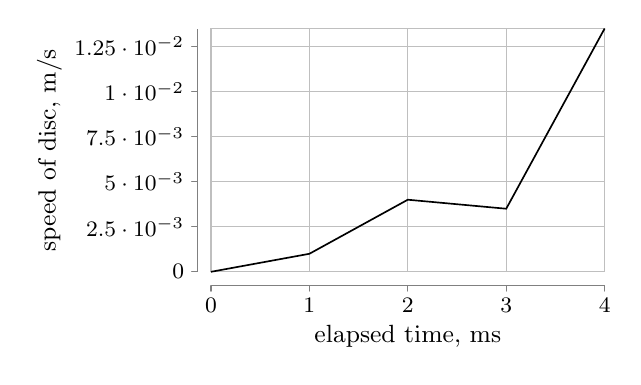
\begin{tikzpicture}
\datavisualization[
	scientific axes=clean,
	x axis={attribute=time,
	label={elapsed time, ms}},
	y axis={attribute=v,
	label={speed of disc, m/s}},
	all axes=grid,
	visualize as line]
data {
	time, v
	0, 0
	1, 0.001
	2, 0.004
	3, 0.0035
	4, 0.0135
};
\end{tikzpicture}
	\end{LTXexample}
	
	\subsection{Figure description}
	\label{figure description}
	Using appropriate vocabulary to describe figure below. Home assignment: plot the figure with \LaTeX:

		\includegraphics[width=0.8\textwidth]{figure1}
	
	Now, erither describe the figure from scratch or just fill-in the  text below (available options are: \textbf{steadily, hovering, trend, meanwhile, rocketed, fluctuated, peak, plummeted, period}):
	
	The chart shows the average daily viewing figures for Channel One News over a 12-month ..................... The figure for the 1pm News remained fairly stable, .................... at around 1.3 million throughout the year. The figure for the 6pm News began the year at 4.8 million. It ...................., but the general .................... was downwards, and it ended the year at 3.4 million.

	The figure for the 9:30 News gradually increased from 3.2 million viewers per day in January to a .................... of 3.8 million in May. However, this month saw the introduction of the 11pm News, and the figure for the 9:30 News ...................., hitting a low-point of 1.1 million in August. In the same period, the figure for the 11pm news .................... from 0.2 million to 4.1 million. At this point, the trend reversed. From August onwards, the figure for the 9:30 news grew ...................., reaching 3 million by the end of the year. ...................., the figure for the 11pm News declined sharply, and in December fell below the 1 million mark.

	\section{Home assignment}
	\subsection{Plotting}
	Plot the figure from Section \ref{figure description} using TikZ package.
	\subsection{Problem Statement}
	Write $\sim$200 words description of your current research problem in \LaTeX.
%	\end{comment}
	\newpage
	\section*{Friday, January 27}
	\section{Scientific paper/thesis writing tips}
	%TODO Include excerpts from The Researcher's Bible, A Brief Guide to Writing a Thesis, Mathematical writing
	
	\subsection{Seven simple suggestions by Simon Peyton Jones}
	
	What follows is mostly applicable to a conference paper, however, some advices are not limited to a particular type of work. Check out the video of the lecture \href{https://youtu.be/g3dkRsTqdDA}{here}.

	\point{Writing papers}
	
	is a primary mechanism for \textit{doing} research, not only reporting/communicating it.
	
	Concepts and ideas are organized clearer when we write. 
	
	\hint{Ideas are not always fantastic; write anyway.} 
	
	Writing is a way of \textit{developing} the idea. It lets you grow the seed-thought into a beautiful flower.
	\medskip
	\begin{center}
	\framebox[1.5\width]{\parbox[b][2em][c]{0.05\textwidth}{Idea}}
	\parbox[b][2em][c]{0.04\textwidth}{$\Longrightarrow$}
	\framebox[1.3\width]{\parbox[b][2em][c]{0.135\textwidth}{Write paper}}
	\parbox[b][2em][c]{0.04\textwidth}{$\Longrightarrow$}
	\framebox[1.3\width]{\parbox[b][2em][c]{0.14\textwidth}{Do research}}
	\end{center}
	
	\point{Key idea}
	
	is useful and reusable. Convey it so that your readers minds are ``infected'' by it - they talk about it and spread it to others. This makes paper a mechanism for conveying the ideas, failing to do this properly kills the idea (no matter how brilliant it is).
	
	\hint{One paper - one clear, sharp idea.} 
	
	When you start it may be hard to articulate the key idea. By the time you finish the paper make sure the reader can clearly understand the bottom line of the paper. If you address several ideas, write several papers!
	
	\hint{Distill the idea.}
	
	Make it clear: ``The main idea of the article is\dots .''
	``In this section we present the main contributions of the paper.''
	
	\point{Tell a story}
	
	in an accessible and engaging way. 
	
	A sample narrative flow can be as follows:
	\begin{itemize}
		\item Here is a problem 
	
		\examplesentence{Machine translation (MT) is hard. Translation deals with natural language which is incredibly reach \dots}
		\item It's an interesting problem 
		 
		\examplesentence{Wouldn't it be nice to have conversations with foreign people without knowing the language? \dots}
		\item It's an unsolved one 
		 
		\examplesentence{So far translation systems have been on a very primitive level. \dots}
		\item Here is my idea 

		\examplesentence{Let's use this approach to MT. \dots}
		\item And it works! (details, data) 
		 
		\examplesentence{I tested my model and got such and such results. \dots}
		\item Here's how my idea compares to other approaches 
		
		\examplesentence{A seminal paper on MT is by Green et al. [1]. It lays the foundation for the work I have done. \dots Blue et al. [2] use very similar approach, however \dots}
	\end{itemize}
	Telling a story is a way to lead the readers into further reading. Most of the people won't read the whole thing, but you should lure them into it. 
	
	\medskip
	Suggested structure:
	\begin{enumerate}
		\item Abstract (4 sentences, 1000 readers)
		\item Introduction (1 page, 100 readers)
		\item The problem (1 page, 10 readers)
		\item My idea (2 page, 10 readers)
		\item The details (5 pages, 3 readers)
		\item Related work (1-2 pages, 10 readers)
		\item Conclusions and further work (half a page)
	\end{enumerate}

	\hint{Introduction: describe the problem briefly\dots} 
	
	Don't give general and obvious descriptions (universal truths), they are boring. 
	%Remember that you need to capture as much attention as possible. 
	Give an instance of the problem to introduce it\footnote{Another hint: in computer science it is often done with a help of a figure. 
	}.
	\href{https://arxiv.org/pdf/1612.01887v1.pdf}{example 1}
	\href{http://www.jmlr.org/proceedings/papers/v48/xiong16.pdf}{example 2}

	
	\point{\dots and state your contributions.}
	
	Write your first draft of contributions early. It drives your paper and research. Once more, be clear: a good thing is to represent your claims as a bulleted list. If the claim failed to be substantiated, simply update the draft with another.
	
	\hint{One bullet - one claim.}
	
	One claim - one forward-reference to the evidence, e.g. section in the paper\footnote{Evidence may be analyses, arguments, measurements, theorems, etc.}. This adds structure and easy navigation across the paper.
	
	\hint{Refutable claims}
	
	Describe contributions as `not easy'. Use actions that might have failed. 
	
	\hint{Unnecessary stuff}
	
	Avoid ``the rest of the paper is structure as follows\dots'' part. Do you ever read it yourself? The structure is given by the forward-references already!
	
	\medskip
	\textit{Example 1 from \href{https://papers.nips.cc/paper/5021-distributed-representations-of-words-and-phrases-and-their-compositionality.pdf}{[Mikolov, 2013]}:}
	
	\medskip
	\textbf{In this paper we present} several extensions of the original Skip-gram model\dots.
	
	First \textbf{we identify} a large number of phrases using a data-driven approach, and then \textbf{we treat} the phrases as individual tokens during the training. To evaluate the quality of the phrase vectors, \textbf{we developed} a test set of analogical reasoning tasks that contains both words and phrases.
	
	\medskip
	\textit{Example 2 from \href{https://arxiv.org/pdf/1612.01887v1.pdf}{[Lu and Xiong, 2016]}:}
	
	\medskip
	\includegraphics[width=0.5\textwidth]{example_contrib}


	\point{Related work}
	
	often forms a barrier between your reader and your idea.
	
	First, keep in mind that you want to bring as many readers as possible into learning about your awesome idea. Most of them would be from a broader field having little knowledge of the notational setup, specifics, intuitions, etc. Because of this lack in background, it would be hard for them to thoroughly comprehend the related work section right after introduction. 
	
	On the one hand, you could make related work very short and dense, so it would be easy to skip for such readers. This approach, however, only scares off the potential reader. 
	
	Alternatively, you can try and build the basics useful to understand ideas from the related work. This only stretches out the section; thereby building a barrier for the potential readers.
	
	Also preceding your idea with related work does not allow for any effective comparison. The reader is not familiar with your solution to the problem. 
	
	The suggestion is to put the related work part just before the end of the paper, i.e. conclusions and further work. 
	\href{http://papers.nips.cc/paper/5346-sequence-to-sequence-learning-with-neural-networks.pdf}{example 1}
	\href{https://arxiv.org/pdf/1612.01887v1.pdf}{example 2}
	\href{http://www.jmlr.org/proceedings/papers/v48/xiong16.pdf}{example 3}
	\href{https://papers.nips.cc/paper/5021-distributed-representations-of-words-and-phrases-and-their-compositionality.pdf}{example 4}
	
	Other tips: give credit when its due, be generous to competition, acknowledge weaknesses.
	
	\point{Readers first}
	
	Make following your ideas easy!
	
	\hint{Intuition first}
	
	Explain the intuition behind the arguments, only then dive into details. Otherwise, lost in notation and specifics, they feel stupid. Treat readers as your friends. Think of how you explained your research to your close friend/relative? Examples! 
	
	%My niece asked me once, what do I do? My research topic is optimization methods for neural networks, so I told her so. Children are inquisitive, so the first thing she asked was `What's an optimization?' this was difficult, really. I tried building up from the graphs like this. But she's only 10! the best explanation was. Imagine your route to school. How many ways can you take to get there? Which one is the fastest? That's it! You try to make the travel time less and this is your own instance of everyday optimization problem.
	
	\hint{Choose the most direct route to the idea.}
	
	\point{Test the paper}

	on your friends. 
	
	\hint{Is it easy to follow/understand?}
	
	Non-experts are also precious since you want to make the paper accessible and engaging! Consider rewriting `I got lost here' parts. Learn how to explain things better.
	
	\hint{Ask for reviews.}
	
	Do not be afraid to receive criticism from experts. If the idea is a rubbish, better find it sooner than later.
	
	\subsection{Some notes regarding thesis writing}
	
	Look at \href{http://www.ifs.tuwien.ac.at/~silvia/research-tips/researchers_bible-1999.pdf}{The Researchers’ Bible} (How to survive a PhD) by Alan Bundy et al. for more.
	
	\hint{Keep working papers and notes as you do your research.}
	
	Some of them can become a publication (journal or conference paper). Collect them into a single folder called ``thesis''. By the time you start building up the text of the thesis,  you will have a material to start working bottom-up: putting together different aspects of your work together.
	
	\hint{Build thesis `message'.}
	
	\begin{itemize}
		\item short (abstract length)
		\item each sentence is a step of an argument. The argument is  the message.
		\item each sentence also aligns with some chapter (outlines its content).
		\item the message is a guide to your thesis.
	\end{itemize}
	Forming a message ensures you thesis is a single coherent piece of work. Also, it helps you understand what should be highlighted in your work. This kind of writing can be called top-down, as you first consider high-level view of the thesis.

	\textit{Example:}
	
	\includegraphics[width=\textwidth]{example_thesis_message}
	
	\section*{References}
	\begin{itemize}
		\item  \href{http://ctan.tug.org/tex-archive/info/lshort/english/lshort.pdf}{A not so short guide to \LaTeX}
		\item \href{http://mirror.macomnet.net/pub/CTAN/graphics/pgf/base/doc/pgfmanual.pdf}{TikZ manual}
		\item \href{http://isites.harvard.edu/fs/docs/icb.topic839892.files/Latex/Skylers_latex_tutorial.pdf}{brief \LaTeX{} tutorial}
		\item \href{http://www.ifs.tuwien.ac.at/~silvia/research-tips/researchers_bible-1999.pdf}{The Researchers’ Bible} (How to survive a PhD) by Alan Bundy et al.
		\item \href{https://www.youtube.com/watch?v=g3dkRsTqdDA}{video} lecture on How to Write a Great Research Paper.
		\item Mathematical thinking \href{http://www-cs-faculty.stanford.edu/~uno/papers/cs1193.pdf}{course lecture notes}, taught by Donal Knuth at Standord.
		\item \href{http://www.vernon.eu/courses/David_Vernon_Writing_a_Thesis.pdf}{A Brief Guide to Writing a Thesis} by David Vernon.
	\end{itemize}
\end{document}